% Options for packages loaded elsewhere
\PassOptionsToPackage{unicode}{hyperref}
\PassOptionsToPackage{hyphens}{url}
%
\documentclass[
]{article}
\usepackage{amsmath,amssymb}
\usepackage{iftex}
\ifPDFTeX
  \usepackage[T1]{fontenc}
  \usepackage[utf8]{inputenc}
  \usepackage{textcomp} % provide euro and other symbols
\else % if luatex or xetex
  \usepackage{unicode-math} % this also loads fontspec
  \defaultfontfeatures{Scale=MatchLowercase}
  \defaultfontfeatures[\rmfamily]{Ligatures=TeX,Scale=1}
\fi
\usepackage{lmodern}
\ifPDFTeX\else
  % xetex/luatex font selection
\fi
% Use upquote if available, for straight quotes in verbatim environments
\IfFileExists{upquote.sty}{\usepackage{upquote}}{}
\IfFileExists{microtype.sty}{% use microtype if available
  \usepackage[]{microtype}
  \UseMicrotypeSet[protrusion]{basicmath} % disable protrusion for tt fonts
}{}
\makeatletter
\@ifundefined{KOMAClassName}{% if non-KOMA class
  \IfFileExists{parskip.sty}{%
    \usepackage{parskip}
  }{% else
    \setlength{\parindent}{0pt}
    \setlength{\parskip}{6pt plus 2pt minus 1pt}}
}{% if KOMA class
  \KOMAoptions{parskip=half}}
\makeatother
\usepackage{xcolor}
\usepackage[margin=1in]{geometry}
\usepackage{color}
\usepackage{fancyvrb}
\newcommand{\VerbBar}{|}
\newcommand{\VERB}{\Verb[commandchars=\\\{\}]}
\DefineVerbatimEnvironment{Highlighting}{Verbatim}{commandchars=\\\{\}}
% Add ',fontsize=\small' for more characters per line
\usepackage{framed}
\definecolor{shadecolor}{RGB}{248,248,248}
\newenvironment{Shaded}{\begin{snugshade}}{\end{snugshade}}
\newcommand{\AlertTok}[1]{\textcolor[rgb]{0.94,0.16,0.16}{#1}}
\newcommand{\AnnotationTok}[1]{\textcolor[rgb]{0.56,0.35,0.01}{\textbf{\textit{#1}}}}
\newcommand{\AttributeTok}[1]{\textcolor[rgb]{0.13,0.29,0.53}{#1}}
\newcommand{\BaseNTok}[1]{\textcolor[rgb]{0.00,0.00,0.81}{#1}}
\newcommand{\BuiltInTok}[1]{#1}
\newcommand{\CharTok}[1]{\textcolor[rgb]{0.31,0.60,0.02}{#1}}
\newcommand{\CommentTok}[1]{\textcolor[rgb]{0.56,0.35,0.01}{\textit{#1}}}
\newcommand{\CommentVarTok}[1]{\textcolor[rgb]{0.56,0.35,0.01}{\textbf{\textit{#1}}}}
\newcommand{\ConstantTok}[1]{\textcolor[rgb]{0.56,0.35,0.01}{#1}}
\newcommand{\ControlFlowTok}[1]{\textcolor[rgb]{0.13,0.29,0.53}{\textbf{#1}}}
\newcommand{\DataTypeTok}[1]{\textcolor[rgb]{0.13,0.29,0.53}{#1}}
\newcommand{\DecValTok}[1]{\textcolor[rgb]{0.00,0.00,0.81}{#1}}
\newcommand{\DocumentationTok}[1]{\textcolor[rgb]{0.56,0.35,0.01}{\textbf{\textit{#1}}}}
\newcommand{\ErrorTok}[1]{\textcolor[rgb]{0.64,0.00,0.00}{\textbf{#1}}}
\newcommand{\ExtensionTok}[1]{#1}
\newcommand{\FloatTok}[1]{\textcolor[rgb]{0.00,0.00,0.81}{#1}}
\newcommand{\FunctionTok}[1]{\textcolor[rgb]{0.13,0.29,0.53}{\textbf{#1}}}
\newcommand{\ImportTok}[1]{#1}
\newcommand{\InformationTok}[1]{\textcolor[rgb]{0.56,0.35,0.01}{\textbf{\textit{#1}}}}
\newcommand{\KeywordTok}[1]{\textcolor[rgb]{0.13,0.29,0.53}{\textbf{#1}}}
\newcommand{\NormalTok}[1]{#1}
\newcommand{\OperatorTok}[1]{\textcolor[rgb]{0.81,0.36,0.00}{\textbf{#1}}}
\newcommand{\OtherTok}[1]{\textcolor[rgb]{0.56,0.35,0.01}{#1}}
\newcommand{\PreprocessorTok}[1]{\textcolor[rgb]{0.56,0.35,0.01}{\textit{#1}}}
\newcommand{\RegionMarkerTok}[1]{#1}
\newcommand{\SpecialCharTok}[1]{\textcolor[rgb]{0.81,0.36,0.00}{\textbf{#1}}}
\newcommand{\SpecialStringTok}[1]{\textcolor[rgb]{0.31,0.60,0.02}{#1}}
\newcommand{\StringTok}[1]{\textcolor[rgb]{0.31,0.60,0.02}{#1}}
\newcommand{\VariableTok}[1]{\textcolor[rgb]{0.00,0.00,0.00}{#1}}
\newcommand{\VerbatimStringTok}[1]{\textcolor[rgb]{0.31,0.60,0.02}{#1}}
\newcommand{\WarningTok}[1]{\textcolor[rgb]{0.56,0.35,0.01}{\textbf{\textit{#1}}}}
\usepackage{graphicx}
\makeatletter
\def\maxwidth{\ifdim\Gin@nat@width>\linewidth\linewidth\else\Gin@nat@width\fi}
\def\maxheight{\ifdim\Gin@nat@height>\textheight\textheight\else\Gin@nat@height\fi}
\makeatother
% Scale images if necessary, so that they will not overflow the page
% margins by default, and it is still possible to overwrite the defaults
% using explicit options in \includegraphics[width, height, ...]{}
\setkeys{Gin}{width=\maxwidth,height=\maxheight,keepaspectratio}
% Set default figure placement to htbp
\makeatletter
\def\fps@figure{htbp}
\makeatother
\setlength{\emergencystretch}{3em} % prevent overfull lines
\providecommand{\tightlist}{%
  \setlength{\itemsep}{0pt}\setlength{\parskip}{0pt}}
\setcounter{secnumdepth}{-\maxdimen} % remove section numbering
\ifLuaTeX
  \usepackage{selnolig}  % disable illegal ligatures
\fi
\usepackage{bookmark}
\IfFileExists{xurl.sty}{\usepackage{xurl}}{} % add URL line breaks if available
\urlstyle{same}
\hypersetup{
  pdftitle={week9HW - Old or fixed data set},
  pdfauthor={Kyle Bosworth},
  hidelinks,
  pdfcreator={LaTeX via pandoc}}

\title{week9HW - Old or fixed data set}
\author{Kyle Bosworth}
\date{2024-10-28}

\begin{document}
\maketitle

{
\setcounter{tocdepth}{2}
\tableofcontents
}
\subsubsection{Load Libraries}\label{load-libraries}

\begin{Shaded}
\begin{Highlighting}[]
\FunctionTok{library}\NormalTok{(here)}
\FunctionTok{library}\NormalTok{(tidyverse)}
\FunctionTok{library}\NormalTok{(dplyr)}
\FunctionTok{library}\NormalTok{(tidyr)}
\FunctionTok{library}\NormalTok{(ggrepel)}
\FunctionTok{library}\NormalTok{(gganimate)}
\FunctionTok{library}\NormalTok{(magick)}
\end{Highlighting}
\end{Shaded}

Read in data: Mullet Guts Project

\begin{Shaded}
\begin{Highlighting}[]
\NormalTok{mgp}\OtherTok{\textless{}{-}}\FunctionTok{read.csv}\NormalTok{(}\FunctionTok{here}\NormalTok{(}\StringTok{"week9"}\NormalTok{,}\StringTok{"data"}\NormalTok{,}\StringTok{"grainsize.csv"}\NormalTok{))}
\FunctionTok{glimpse}\NormalTok{(mgp)}
\end{Highlighting}
\end{Shaded}

\begin{verbatim}
## Rows: 79
## Columns: 20
## $ Date          <chr> "2022-10-01", "2022-10-01", "2022-10-01", "2022-10-01", ~
## $ Site.Name     <chr> "MS-B9", "MS-B10", "MS-B11", "ME-B13", "ME-B14", NA, "MN~
## $ Alt.site.name <chr> "P-01", "P-02", "P-03", "P-04", "P-05", "P-06", "P-07", ~
## $ Zone          <chr> "Mullet South", "Mullet South", "Mullet South", "Mullet ~
## $ Lat           <dbl> 21.43225, 21.43336, 21.43438, 21.43591, 21.43704, 21.439~
## $ Long          <dbl> -157.8067, -157.8062, -157.8053, -157.8056, -157.8061, -~
## $ TotalWeight   <dbl> 36.708, 36.539, 59.917, 44.272, 58.144, 36.614, 35.681, ~
## $ Total.        <int> 100, 100, 100, 100, 100, 100, 100, 100, 100, 100, 100, 1~
## $ Gravel        <dbl> 12.271, 32.646, 29.637, 39.237, 19.361, 13.160, 8.952, 6~
## $ CoarseSand    <dbl> 11.226, 21.761, 22.837, 40.258, 29.697, 15.923, 6.944, 7~
## $ MediumSand    <dbl> 13.972, 9.925, 9.878, 9.724, 9.900, 5.271, 6.419, 9.832,~
## $ FineSand      <dbl> 18.741, 24.244, 18.066, 6.388, 18.589, 15.953, 28.968, 2~
## $ SiltClay      <dbl> 43.791, 11.424, 19.582, 4.392, 22.454, 49.693, 48.716, 4~
## $ TempC         <dbl> 25.300, 26.200, 27.400, 27.600, 27.800, 27.400, 27.200, ~
## $ DO.           <dbl> 28.3, 34.9, 59.5, 80.8, 100.9, 67.1, 46.8, 63.0, 41.8, 3~
## $ DO            <chr> "1.95", "2.37", "3.89", "5.25", "6.52", "4.4", "3.12", "~
## $ SpC           <dbl> 47.985, 48.185, 52.181, 52.832, 53.004, 50.854, 48.194, ~
## $ Salinity      <dbl> 31.26, 31.38, 34.28, 34.76, 34.88, 33.30, 31.36, 29.63, ~
## $ pH            <dbl> 7.83, 7.92, 7.99, 8.20, 8.25, 7.90, 7.90, 7.82, 7.80, 7.~
## $ Turbidity     <dbl> 0.71, 0.75, 0.99, 0.88, 0.80, 2.44, 1.88, 3.42, 1.05, 0.~
\end{verbatim}

Old data set: Total percent grain size will not equal \%100 Updated data
set, Total grainsize \% = 100

Function 1. Check grain size \% adds up to 100?

\begin{Shaded}
\begin{Highlighting}[]
\NormalTok{check\_grain\_size\_percent}\OtherTok{\textless{}{-}} \ControlFlowTok{function}\NormalTok{(SiltClay, FineSand, MediumSand, CoarseSand, Gravel, TotalWeight) }\CommentTok{\#arguments }
\NormalTok{\{ }\CommentTok{\# need to combine all percentages}
\NormalTok{  percentages}\OtherTok{\textless{}{-}} \FunctionTok{c}\NormalTok{(SiltClay, FineSand, MediumSand, CoarseSand, Gravel)}
  
  \CommentTok{\# calculate sum using percentages}
\NormalTok{  total}\OtherTok{\textless{}{-}} \FunctionTok{sum}\NormalTok{(percentages, }\AttributeTok{na.rm =} \ConstantTok{TRUE}\NormalTok{)}
  
  \CommentTok{\# checking if the sum is close to 100, allowing for a small rounding error}
   \ControlFlowTok{if}\NormalTok{ (}\SpecialCharTok{!}\FunctionTok{any}\NormalTok{(}\FunctionTok{is.na}\NormalTok{(percentages))) \{}
    \ControlFlowTok{if}\NormalTok{ (}\FunctionTok{abs}\NormalTok{(total }\SpecialCharTok{{-}} \DecValTok{100}\NormalTok{) }\SpecialCharTok{\textgreater{}} \DecValTok{1}\NormalTok{) \{}
      \FunctionTok{warning}\NormalTok{(}\FunctionTok{paste}\NormalTok{(}\StringTok{"Total percentage is"}\NormalTok{, total, }\StringTok{"which is not close to 100. Check your data."}\NormalTok{))}
\NormalTok{    \}}
\NormalTok{  \} }\ControlFlowTok{else}\NormalTok{ \{}
    \FunctionTok{warning}\NormalTok{(}\StringTok{"NA values present in the data."}\NormalTok{)}
\NormalTok{  \}}
  
  \CommentTok{\# Now return the percentages as a data fram}
  \FunctionTok{data.frame}\NormalTok{(}
    \AttributeTok{SiltClay\_percent =}\NormalTok{ SiltClay,}
    \AttributeTok{FineSand\_percent =}\NormalTok{ FineSand,}
    \AttributeTok{MediumSand\_percent =}\NormalTok{ MediumSand,}
    \AttributeTok{CoarseSand\_percent =}\NormalTok{ CoarseSand,}
    \AttributeTok{Gravel\_percent =}\NormalTok{ Gravel,}
    \AttributeTok{Total =}\NormalTok{ total}
\NormalTok{  )}
\NormalTok{\}}
\CommentTok{\# adding new percentages and the total percent \% columns}
\CommentTok{\# pmap is used to apply the checked\_grain\_size\_percent function to each orw of the data frame}

\NormalTok{mgp }\OtherTok{\textless{}{-}}\NormalTok{ mgp }\SpecialCharTok{\%\textgreater{}\%}
  \FunctionTok{mutate}\NormalTok{(}\AttributeTok{checked\_percentages =} \FunctionTok{pmap}\NormalTok{(}\FunctionTok{list}\NormalTok{(SiltClay, FineSand, MediumSand, CoarseSand, Gravel),}
\NormalTok{                                    check\_grain\_size\_percent))}

\CommentTok{\# Unnest the results to see the total \% = 100?}
\NormalTok{mgp }\OtherTok{\textless{}{-}}\NormalTok{ mgp }\SpecialCharTok{\%\textgreater{}\%}
  \FunctionTok{unnest}\NormalTok{(checked\_percentages)}

\FunctionTok{glimpse}\NormalTok{(mgp)}
\end{Highlighting}
\end{Shaded}

\begin{verbatim}
## Rows: 79
## Columns: 26
## $ Date               <chr> "2022-10-01", "2022-10-01", "2022-10-01", "2022-10-~
## $ Site.Name          <chr> "MS-B9", "MS-B10", "MS-B11", "ME-B13", "ME-B14", NA~
## $ Alt.site.name      <chr> "P-01", "P-02", "P-03", "P-04", "P-05", "P-06", "P-~
## $ Zone               <chr> "Mullet South", "Mullet South", "Mullet South", "Mu~
## $ Lat                <dbl> 21.43225, 21.43336, 21.43438, 21.43591, 21.43704, 2~
## $ Long               <dbl> -157.8067, -157.8062, -157.8053, -157.8056, -157.80~
## $ TotalWeight        <dbl> 36.708, 36.539, 59.917, 44.272, 58.144, 36.614, 35.~
## $ Total.             <int> 100, 100, 100, 100, 100, 100, 100, 100, 100, 100, 1~
## $ Gravel             <dbl> 12.271, 32.646, 29.637, 39.237, 19.361, 13.160, 8.9~
## $ CoarseSand         <dbl> 11.226, 21.761, 22.837, 40.258, 29.697, 15.923, 6.9~
## $ MediumSand         <dbl> 13.972, 9.925, 9.878, 9.724, 9.900, 5.271, 6.419, 9~
## $ FineSand           <dbl> 18.741, 24.244, 18.066, 6.388, 18.589, 15.953, 28.9~
## $ SiltClay           <dbl> 43.791, 11.424, 19.582, 4.392, 22.454, 49.693, 48.7~
## $ TempC              <dbl> 25.300, 26.200, 27.400, 27.600, 27.800, 27.400, 27.~
## $ DO.                <dbl> 28.3, 34.9, 59.5, 80.8, 100.9, 67.1, 46.8, 63.0, 41~
## $ DO                 <chr> "1.95", "2.37", "3.89", "5.25", "6.52", "4.4", "3.1~
## $ SpC                <dbl> 47.985, 48.185, 52.181, 52.832, 53.004, 50.854, 48.~
## $ Salinity           <dbl> 31.26, 31.38, 34.28, 34.76, 34.88, 33.30, 31.36, 29~
## $ pH                 <dbl> 7.83, 7.92, 7.99, 8.20, 8.25, 7.90, 7.90, 7.82, 7.8~
## $ Turbidity          <dbl> 0.71, 0.75, 0.99, 0.88, 0.80, 2.44, 1.88, 3.42, 1.0~
## $ SiltClay_percent   <dbl> 43.791, 11.424, 19.582, 4.392, 22.454, 49.693, 48.7~
## $ FineSand_percent   <dbl> 18.741, 24.244, 18.066, 6.388, 18.589, 15.953, 28.9~
## $ MediumSand_percent <dbl> 13.972, 9.925, 9.878, 9.724, 9.900, 5.271, 6.419, 9~
## $ CoarseSand_percent <dbl> 11.226, 21.761, 22.837, 40.258, 29.697, 15.923, 6.9~
## $ Gravel_percent     <dbl> 12.271, 32.646, 29.637, 39.237, 19.361, 13.160, 8.9~
## $ Total              <dbl> 100.001, 100.000, 100.000, 99.999, 100.001, 100.000~
\end{verbatim}

\begin{Shaded}
\begin{Highlighting}[]
\FunctionTok{view}\NormalTok{(mgp)}
\end{Highlighting}
\end{Shaded}

There are some that do not add up to 100\%, must be old data.

Function 2 with plot: identify error rows and plot

\begin{Shaded}
\begin{Highlighting}[]
\CommentTok{\#function that identifies rows that don\textquotesingle{}t sum to 100}
\NormalTok{identify\_not100 }\OtherTok{\textless{}{-}} \ControlFlowTok{function}\NormalTok{(data, grain\_columns, }\AttributeTok{tolerance =} \DecValTok{1}\NormalTok{) \{}
\NormalTok{  data }\SpecialCharTok{\%\textgreater{}\%}
    \CommentTok{\#calculating the total of all grain size columns for each row}
    \FunctionTok{mutate}\NormalTok{(}\AttributeTok{total =} \FunctionTok{rowSums}\NormalTok{(}\FunctionTok{select}\NormalTok{(., }\FunctionTok{all\_of}\NormalTok{(grain\_columns)), }\AttributeTok{na.rm =} \ConstantTok{TRUE}\NormalTok{),}
           \CommentTok{\#need to create a logical column, TRUE if the total isnʻt in the tolerance of 100}
           \AttributeTok{isnot100 =} \FunctionTok{abs}\NormalTok{(total }\SpecialCharTok{{-}} \DecValTok{100}\NormalTok{) }\SpecialCharTok{\textgreater{}}\NormalTok{ tolerance) }\SpecialCharTok{\%\textgreater{}\%}
    \CommentTok{\#keeping only the rows where isnot100 is TURE}
    \FunctionTok{filter}\NormalTok{(isnot100)}
\NormalTok{\}}

\CommentTok{\#function to plot grain size distribution for a single sample}
\NormalTok{plot\_grain\_size }\OtherTok{\textless{}{-}} \ControlFlowTok{function}\NormalTok{(data, site\_name\_col, date\_col, grain\_columns) \{}
\NormalTok{  data\_long }\OtherTok{\textless{}{-}}\NormalTok{ data }\SpecialCharTok{\%\textgreater{}\%}
    \CommentTok{\#reshape to long format }
    \CommentTok{\#selecting only these columns}
    \FunctionTok{select}\NormalTok{(}\FunctionTok{all\_of}\NormalTok{(}\FunctionTok{c}\NormalTok{(site\_name\_col, date\_col, grain\_columns))) }\SpecialCharTok{\%\textgreater{}\%}
   
    \CommentTok{\#convert grainsize columns into two, Grainsize ad Percentage}
     \FunctionTok{pivot\_longer}\NormalTok{(}\AttributeTok{cols =} \FunctionTok{all\_of}\NormalTok{(grain\_columns),}
                 \AttributeTok{names\_to =} \StringTok{"GrainSize"}\NormalTok{, }
                 \AttributeTok{values\_to =} \StringTok{"Percentage"}\NormalTok{)}
  \CommentTok{\#making ggplot }
  \FunctionTok{ggplot}\NormalTok{(data\_long, }
         \FunctionTok{aes}\NormalTok{(}\AttributeTok{x =}\NormalTok{ GrainSize,}\CommentTok{\#grainsize categories}
             \AttributeTok{y =}\NormalTok{ Percentage, }\CommentTok{\#percentage values}
             \AttributeTok{fill =}\NormalTok{ GrainSize)) }\SpecialCharTok{+} \CommentTok{\#coor by grainsize cat.}
    
    \FunctionTok{geom\_bar}\NormalTok{(}\AttributeTok{stat =} \StringTok{"identity"}\NormalTok{) }\SpecialCharTok{+} \CommentTok{\#add bars}
    \FunctionTok{geom\_text}\NormalTok{(}\FunctionTok{aes}\NormalTok{(}\AttributeTok{label =} \FunctionTok{round}\NormalTok{(Percentage, }\DecValTok{1}\NormalTok{)), }\AttributeTok{vjust =} \SpecialCharTok{{-}}\FloatTok{0.5}\NormalTok{) }\SpecialCharTok{+} \CommentTok{\#add bar labels}
    \FunctionTok{theme\_minimal}\NormalTok{() }\SpecialCharTok{+}
    
  \CommentTok{\#add titles/labels  }
    
    \FunctionTok{labs}\NormalTok{(}\AttributeTok{title =} \FunctionTok{paste}\NormalTok{(}\StringTok{"Grain Size Distribution for Site"}\NormalTok{, data[[site\_name\_col]], }\StringTok{"on"}\NormalTok{, data[[date\_col]]),}
         
         \AttributeTok{subtitle =} \FunctionTok{paste}\NormalTok{(}\StringTok{"Total:"}\NormalTok{, }\FunctionTok{sum}\NormalTok{(data\_long}\SpecialCharTok{$}\NormalTok{Percentage, }\AttributeTok{na.rm =} \ConstantTok{TRUE}\NormalTok{), }\StringTok{"\%"}\NormalTok{),}
         \AttributeTok{x =} \StringTok{"Grain Size"}\NormalTok{, }
         \AttributeTok{y =} \StringTok{"Percentage"}\NormalTok{) }\SpecialCharTok{+}
    \FunctionTok{theme}\NormalTok{(}\AttributeTok{axis.text.x =} \FunctionTok{element\_text}\NormalTok{(}\AttributeTok{angle =} \DecValTok{45}\NormalTok{, }\AttributeTok{hjust =} \DecValTok{1}\NormalTok{)) }\CommentTok{\#rotate axis labels}
\NormalTok{\}}

\CommentTok{\# Specify your column names fr Grain sizes}
\NormalTok{grain\_columns }\OtherTok{\textless{}{-}} \FunctionTok{c}\NormalTok{(}\StringTok{"SiltClay"}\NormalTok{, }\StringTok{"FineSand"}\NormalTok{, }\StringTok{"MediumSand"}\NormalTok{, }\StringTok{"CoarseSand"}\NormalTok{, }\StringTok{"Gravel"}\NormalTok{)}

\NormalTok{site\_name\_col }\OtherTok{\textless{}{-}} \StringTok{"Site.Name"}  \CommentTok{\#site identification column name}

\NormalTok{date\_col }\OtherTok{\textless{}{-}} \StringTok{"Date"}  \CommentTok{\#date column name}


\CommentTok{\# Identify samples that don\textquotesingle{}t equal 100\%}
\NormalTok{non\_100\_samples }\OtherTok{\textless{}{-}} \FunctionTok{identify\_not100}\NormalTok{(mgp, grain\_columns)}

\CommentTok{\# create a list of each plot, one is fo each not = 100\% sample}
\NormalTok{plot\_list }\OtherTok{\textless{}{-}} \FunctionTok{lapply}\NormalTok{(}\DecValTok{1}\SpecialCharTok{:}\FunctionTok{nrow}\NormalTok{(non\_100\_samples), }\ControlFlowTok{function}\NormalTok{(i) \{}
  \FunctionTok{plot\_grain\_size}\NormalTok{(non\_100\_samples[i,], site\_name\_col, date\_col, grain\_columns)}
\NormalTok{\})}

\CommentTok{\#display each of the plots in the list}
\ControlFlowTok{for}\NormalTok{ (plot }\ControlFlowTok{in}\NormalTok{ plot\_list) \{}
  \FunctionTok{print}\NormalTok{(plot)}
\NormalTok{\}}
\end{Highlighting}
\end{Shaded}

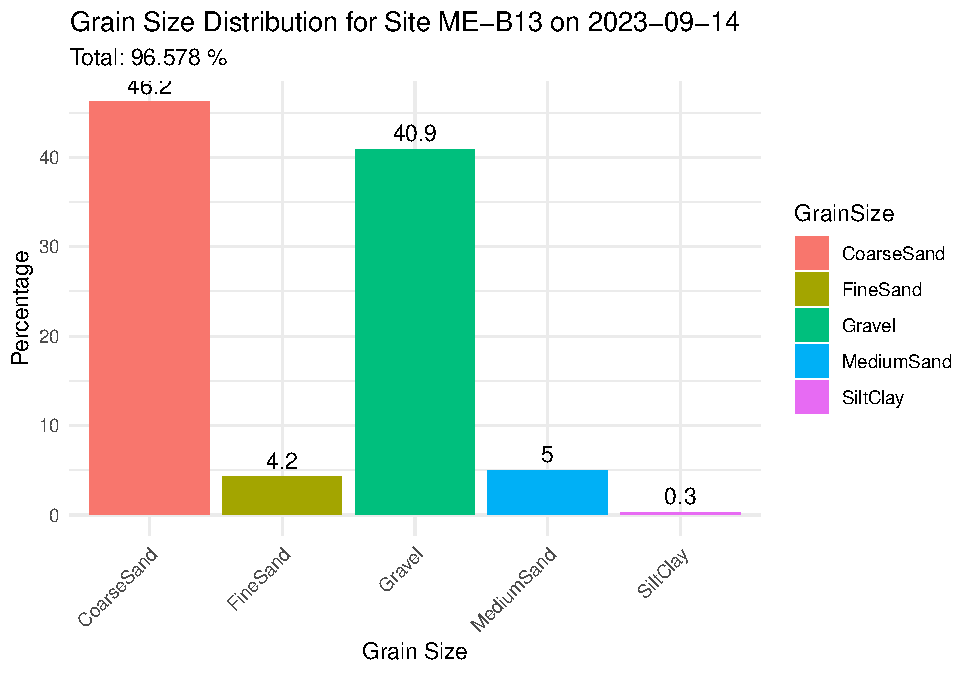
\includegraphics{week9HWa_files/figure-latex/unnamed-chunk-4-1.pdf}
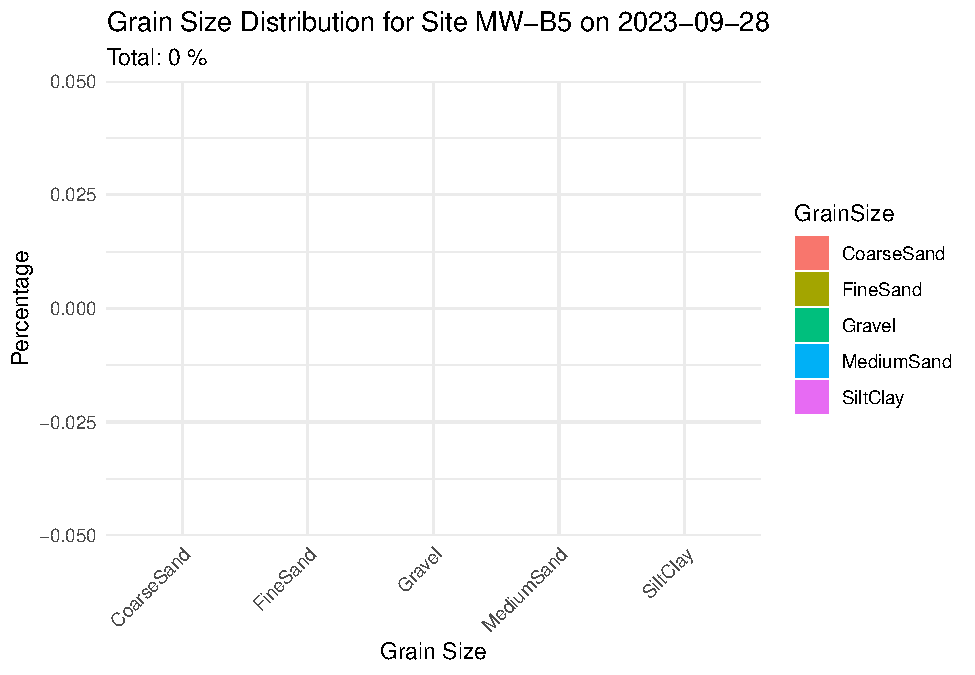
\includegraphics{week9HWa_files/figure-latex/unnamed-chunk-4-2.pdf}
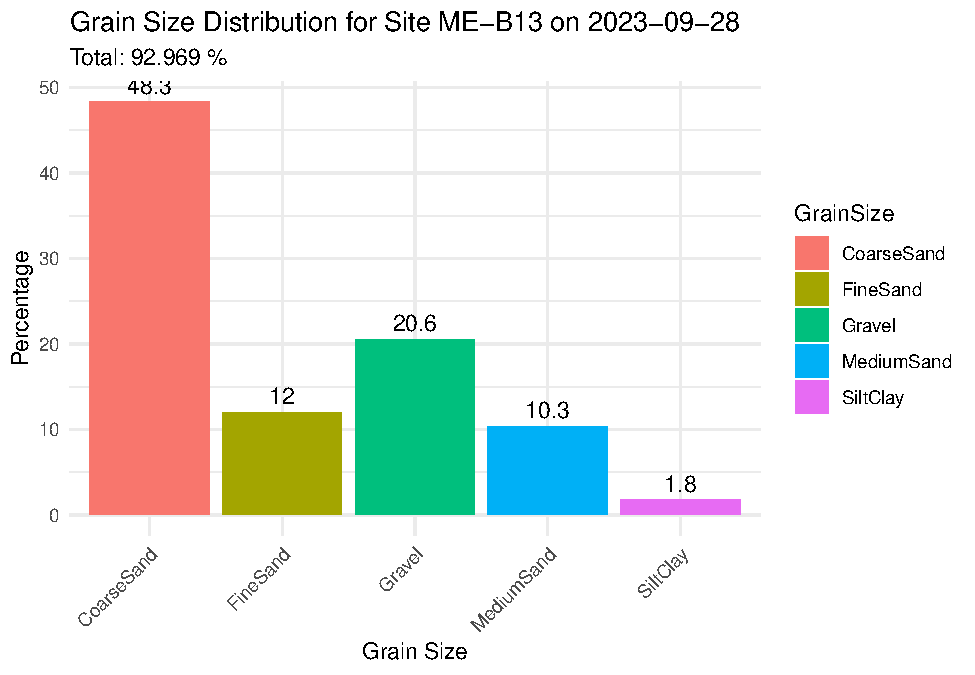
\includegraphics{week9HWa_files/figure-latex/unnamed-chunk-4-3.pdf}
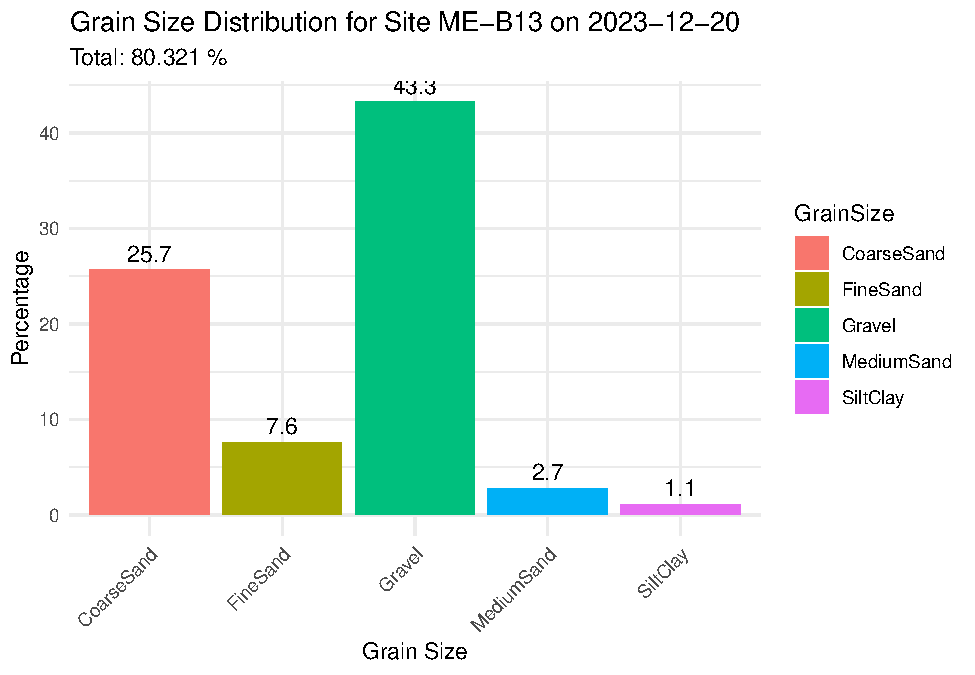
\includegraphics{week9HWa_files/figure-latex/unnamed-chunk-4-4.pdf}

\end{document}
